% =====================================================================
%  OTT 串流平台二維動態策略模型 — 課程簡報 (Beamer)
%  Source: OTT_strategy_model_report-2.pdf  (Information Economics & Game Theory, 2026)
%  Engine: XeLaTeX  (CJK via ctexbeamer + PingFang TC)
%  Build:  xelatex OTT_strategy_slides.tex   (run twice: TOC + page counter + grid bg)
%  Theme:  royal-blue + grid-paper background (per the user's template)
% =====================================================================
\documentclass[aspectratio=169,11pt,fontset=none]{ctexbeamer}

% ---------- CJK fonts (Traditional Chinese, macOS) ----------
\setCJKmainfont{PingFang TC}
\setCJKsansfont{PingFang TC}
\setCJKmonofont{Heiti TC}

% ---------- packages (TeX Live "basic": built-in beamer + tikz only) ----------
\usepackage{amsmath,amssymb}
\usepackage{pifont}        % \ding check/cross marks
\usepackage{tikz}
\usetikzlibrary{arrows.meta,positioning}
\usepackage{graphicx}
\graphicspath{{./}}

% ---------- colour palette ----------
% theme = royal blue (from the user's template); data colours = the 4 strategy cells
\definecolor{rblue}{HTML}{2B4CC9}     % primary royal blue
\definecolor{rnavy}{HTML}{1E3A82}     % deep navy accent
\definecolor{gridc}{HTML}{DCE3F3}     % light grid-paper lines
\definecolor{ottred}{HTML}{E63946}    % Trans-Acq
\definecolor{ottorange}{HTML}{F4A261} % Trans-Ret
\definecolor{ottteal}{HTML}{2A9D8F}   % Sub-Acq
\definecolor{ottdark}{HTML}{264653}   % Sub-Ret
\definecolor{ottsand}{HTML}{E9C46A}
\definecolor{ottgray}{HTML}{6B7B82}

% ---------- clean self-rolled theme (no external theme packages) ----------
\usetheme{default}
\useinnertheme{circles}
\setbeamertemplate{navigation symbols}{}
\setbeamercolor{structure}{fg=rblue}
\setbeamercolor{title}{fg=rblue}
\setbeamercolor{frametitle}{fg=rblue,bg=}
\setbeamercolor{itemize item}{fg=rblue}
\setbeamercolor{itemize subitem}{fg=rblue}
\setbeamercolor{enumerate item}{fg=rblue}
\setbeamercolor{block title}{fg=white,bg=rblue}
\setbeamercolor{block body}{fg=black,bg=rblue!7}
\setbeamercolor{block title alerted}{fg=white,bg=ottred}
\setbeamercolor{block body alerted}{fg=black,bg=ottred!8}
\setbeamercolor{block title example}{fg=white,bg=ottteal}
\setbeamercolor{block body example}{fg=black,bg=ottteal!9}
\setbeamerfont{frametitle}{series=\bfseries,size=\large}
\setbeamerfont{title}{series=\bfseries,size=\LARGE}
\setbeamerfont{block title}{series=\bfseries}

% grid-paper background on every slide
\setbeamertemplate{background}{%
  \begin{tikzpicture}[remember picture,overlay]
    \fill[white] (current page.south west) rectangle (current page.north east);
    \draw[gridc,line width=0.3pt,step=0.5cm]
      (current page.south west) grid (current page.north east);
  \end{tikzpicture}}

% frame title: blue, with a thin blue underline rule
\setbeamertemplate{frametitle}{%
  \nointerlineskip\vskip0.5em
  {\usebeamerfont{frametitle}\usebeamercolor[fg]{frametitle}\insertframetitle\par}%
  \vskip2pt{\color{rblue!55}\rule{\textwidth}{0.7pt}}\par}

% minimal blue footline: title | author | frame number
\setbeamercolor{footcolor}{fg=white,bg=rblue}
\setbeamertemplate{footline}{%
  \leavevmode\hbox{%
    \begin{beamercolorbox}[wd=\paperwidth,ht=2.6ex,dp=1.1ex,leftskip=1.2em,rightskip=1.2em]{footcolor}%
      \footnotesize OTT 二維動態策略模型\hfill\insertshortauthor\hfill\insertframenumber\,/\,\inserttotalframenumber
    \end{beamercolorbox}}%
}

% TOC entries: big blue section number + title; fade non-current on dividers
\setbeamerfont{section in toc}{size=\large}
\setbeamercolor{section in toc}{fg=black}
\setbeamertemplate{section in toc}{%
  \leavevmode{\color{rblue}\bfseries\inserttocsectionnumber.}\hspace{0.7em}\inserttocsection\par\medskip}
\setbeamertemplate{section in toc shaded}[default][40]

% section divider = highlighted two-column table of contents
\AtBeginSection[]{%
  \begin{frame}{大綱}
    \vfill
    \begin{columns}[T]
      \column{0.48\textwidth}
        \tableofcontents[currentsection,sections={1-3},sectionstyle=show/shaded]
      \column{0.48\textwidth}
        \tableofcontents[currentsection,sections={4-6},sectionstyle=show/shaded]
    \end{columns}
    \vfill
  \end{frame}}

% ---------- small helpers ----------
\newcommand{\chip}[1]{\tikz[baseline=-0.5ex]\node[fill=#1,inner sep=2.6pt,rounded corners=1pt]{};}
\newcommand{\hl}[1]{{\color{rblue}\bfseries #1}}
\newcommand{\rd}[1]{{\color{ottred}\bfseries #1}}
\newcommand{\TA}{\textcolor{ottred}{\textbf{Trans-Acq}}}
\newcommand{\TR}{\textcolor{ottorange}{\textbf{Trans-Ret}}}
\newcommand{\SA}{\textcolor{ottteal}{\textbf{Sub-Acq}}}
\newcommand{\SR}{\textcolor{ottdark}{\textbf{Sub-Ret}}}

% ---------- title metadata ----------
\title{線上影音串流平台之\\二維動態策略模型}
\subtitle{收費模式選擇 $\times$ 客群策略 $\times$ 市佔率動態}
\author[IEGT 2026]{報告團隊}             % TODO: 替換為實際報告人姓名
\institute{Information Economics and Game Theory $\cdot$ 課程研究報告}
\date{2026}

% =====================================================================
\begin{document}

% ----------------------------- Title -----------------------------
{\setbeamertemplate{footline}{}
\begin{frame}[plain]
  \vfill
  \begin{center}
    {\color{rblue}\rule{0.66\textwidth}{1.6pt}}\\[0.8em]
    {\usebeamerfont{title}\usebeamercolor[fg]{title}\inserttitle\par}\vskip0.35em
    {\large\color{ottgray} A Two-Dimensional Dynamic Strategic Model for OTT Platforms}\\[0.7em]
    {\color{rblue}\rule{0.66\textwidth}{1.6pt}}\\[1.0em]
    {\large\insertsubtitle\par}\vskip1.3em
    {\footnotesize 方法論模板:Erickson (1992);Rhouma \& Zaccour (2018)}\\[0.3em]
    {\insertinstitute\ $\cdot$ \insertdate}
  \end{center}
  \vfill
\end{frame}}

% ----------------------------- Table of contents -----------------------------
\begin{frame}
  \vskip0.3em
  \begin{center}
    {\fontsize{26}{30}\selectfont\color{rblue}\bfseries Table of contents}
  \end{center}
  \vskip0.2em{\color{rblue!55}\rule{\textwidth}{0.7pt}}
  \vfill
  \begin{columns}[T]
    \column{0.48\textwidth}\tableofcontents[sections={1-3}]
    \column{0.48\textwidth}\tableofcontents[sections={4-6}]
  \end{columns}
  \vfill
\end{frame}

% =====================================================================
\section{研究背景與動機}
% =====================================================================

\begin{frame}{研究背景:OTT 平台的兩個根本決策}
  OTT(Over-The-Top)串流平台的兩個核心策略,皆與當前市佔率 $s$ 密切相關:
  \begin{columns}[t]
    \column{0.5\textwidth}
      \begin{block}{收費模式 $P$}
        \footnotesize
        \textbf{S} = 訂閱制 SVOD(Netflix 月費吃到飽)\\
        \textbf{T} = 單部購買 TVOD(iTunes 單片租購)
      \end{block}
    \column{0.5\textwidth}
      \begin{block}{客群策略 $C$}
        \footnotesize
        \textbf{A} = 新客獲取 Acquisition(廣告、試用)\\
        \textbf{R} = 舊客保留 Retention(推薦、折扣、內容)
      \end{block}
  \end{columns}
  \vskip0.3em
  \begin{center}\small
  \begin{tabular}{c|cc}
     & $C=A$(獲取) & $C=R$(保留)\\\hline
    $P=T$(TVOD) & \chip{ottred}\ \textcolor{ottred}{\textbf{Trans-Acq}} & \chip{ottorange}\ \textcolor{ottorange}{\textbf{Trans-Ret}}\\
    $P=S$(SVOD) & \chip{ottteal}\ \textcolor{ottteal}{\textbf{Sub-Acq}} & \chip{ottdark}\ \textcolor{ottdark}{\textbf{Sub-Ret}}\\
  \end{tabular}
  \end{center}
  \begin{alertblock}{核心問題}
    給定 $s$,廠商應如何在 4 種組合 $(P,C)\in\{T,S\}\times\{A,R\}$ 中選擇,
    以最大化跨期折現利潤?最適策略如何\textbf{隨 $s$ 變化}?
  \end{alertblock}
\end{frame}

\begin{frame}{研究問題與方法論定位}
  \begin{itemize}
    \item \hl{框架}:單一廠商、無限期、折現的動態最佳化(Bellman / value iteration)。
    \item \hl{狀態變數}:市佔率 $s\in[0,1]$ —— 外生演化的單一狀態。
    \item \hl{控制變數}:策略組合 $(P,C)$ —— 每期同時選擇兩個維度。
  \end{itemize}
  \vskip0.3em
  \begin{block}{為何這樣定位}
    研究問題聚焦「\textbf{給定 $s$,單一廠商如何選}」,而非「市場均衡是什麼」。
    單一廠商假設使策略地圖乾淨,並將競爭壓力透過\textbf{市場飽和效應}與
    \textbf{留存率上限}內生反映;完整競爭擴展留待第 5 章(Stackelberg)。
  \end{block}
  \vskip0.2em
  {\footnotesize 對照:Bernstein et al. (2022) 用「信念」作 state;本研究用「市佔率 $s$」,
   因 $s$ 同時驅動收入規模與轉移動態,更貼近 OTT 經營語言。}
\end{frame}

% =====================================================================
\section{文獻回顧}
% =====================================================================

\begin{frame}{兩條成熟但分離的文獻流}
  \begin{columns}[t]
    \column{0.5\textwidth}
      \begin{block}{Stream 1:收費模式選擇}
        \footnotesize
        資訊財定價(Sundararajan 2004;Bakos--Brynjolfsson 1999;Rao 2015)\\[0.2em]
        $\to$ SVOD vs.\ TVOD 的最適選擇,但多為\textbf{靜態},且不涉及客群策略。
      \end{block}
    \column{0.5\textwidth}
      \begin{block}{Stream 2:客群策略}
        \footnotesize
        行銷科學(Rhouma--Zaccour 2018;Erickson 1992;Gupta et al.\ 2004)\\[0.2em]
        $\to$ acquisition vs.\ retention 動態配置,但\textbf{不涉及收費模式}。
      \end{block}
  \end{columns}
  \vskip0.4em
  \begin{alertblock}{文獻缺口}
    兩條 stream 各自成熟,\textbf{但兩者的整合仍是空白}:Rhouma--Zaccour 不含收費模式;
    Bernstein et al.\ (2022) 收費模式固定為 SVOD;Rao (2015) 是靜態。
  \end{alertblock}
  \vskip0.2em
  {\footnotesize 關鍵校準來源:Iyengar et al.\ (2011,$\delta_S$);Datta et al.\ (2015,free-trial CLV);
   Reinartz et al.\ (2005,投入配比)。}
\end{frame}

\begin{frame}{本研究的貢獻:在同一 Bellman 框架下整合}
  \begin{exampleblock}{「整合」本身即是貢獻}
    以\hl{市佔率 $s$ 作為共同狀態變數},把動態 acquisition/retention(Rhouma--Zaccour 傳統)
    與資訊財收費模式選擇(Bakos--Brynjolfsson 傳統)整合進同一個 Bellman 框架。
  \end{exampleblock}
  \vskip0.3em
  \begin{block}{關鍵耦合機制(既有文獻所無)}
    讓收費模式 $P$ \textbf{同時影響}留存率 $\rho$ 與獲取率 $\alpha$:
    \begin{itemize}\footnotesize
      \item SVOD 天生有利於 \textbf{retention}(flat-rate usage 與留存正相關;Iyengar 2011)。
      \item TVOD 較有利於 \textbf{acquisition}(無 commitment,拉新門檻低;Rao 2015)。
      \item 市佔率 $s$ 驅動收費模式轉換(nascent $\to$ mature;Sundararajan 2004)。
    \end{itemize}
  \end{block}
  {\footnotesize 每條 stream 單獨而言無方法論創新;貢獻在於\textbf{整合}與整合後浮現的非平凡性質。}
\end{frame}

% =====================================================================
\section{模型建構}
% =====================================================================

\begin{frame}{環境設定與行動空間}
  \begin{columns}[t]
    \column{0.54\textwidth}
      \begin{itemize}
        \item 單一廠商,離散時間 $t=0,1,2,\dots$
        \item 無限期 $+$ 折現,折現因子 $\beta=0.95$
        \item 潛在市場標準化為 $1$;市佔率 $s_t\in[0,1]$
        \item 非用戶池 $1-s_t$:可被獲取的潛在客戶
        \item 行動 $a=(P,C)$,離散集合 $\mathcal{A}$ 共 4 個 cell
      \end{itemize}
      \vskip0.5em
      {\footnotesize 時序:期初 $s_t$ $\to$ 本期收入基於 $s_t$ $\to$ 期內流失與新獲取
       $\to$ 期末 $s_{t+1}$。Markov 轉移:$s_{t+1}$ 只依 $(s_t,a_t)$。}
    \column{0.46\textwidth}
      \begin{block}{$2\times2$ 行動集合}
        \centering
        \begin{tabular}{c|cc}
          & $C=A$ & $C=R$\\\hline
          $P=T$ & \chip{ottred} TA & \chip{ottorange} TR\\
          $P=S$ & \chip{ottteal} SA & \chip{ottdark} SR\\
        \end{tabular}
      \end{block}
      \begin{block}{價格外生}
        $p_S=15$,$p_T=5$ 為業界標準,廠商不調價。
      \end{block}
  \end{columns}
\end{frame}

\begin{frame}{利潤函數(Stage Profit)}
  \[
    \pi(s,a)=\underbrace{R(s,P)}_{\text{每用戶收入}}\cdot\, s \;-\; \underbrace{C(C)}_{\text{行銷成本}}
  \]
  \begin{columns}[t]
    \column{0.5\textwidth}
      \begin{block}{收入函數 $R(s,P)$}
        \[
          R(s,P)=\begin{cases} p_S = 15 & P=S\\[0.3em]
          p_T(\varphi_0+\varphi_1 s)=2.5+2.5s & P=T\end{cases}
        \]
        \footnotesize SVOD:規模\textbf{無感}的均一收費。\\
        TVOD:規模\textbf{敏感}—平台越大、人均購買頻率越高。\\
        校準方向 $R(s,S)>R(s,T)\ \forall s$。
      \end{block}
    \column{0.5\textwidth}
      \begin{block}{成本函數 $C(C)$}
        \[ C(C)=\begin{cases} c_A=1.2 & C=A\\ c_R=0.8 & C=R\end{cases} \]
        \footnotesize \textbf{校準誠實性}:$c_A>c_R$ 是{\color{ottred}方向性}結論
        ——「執行一次該策略的固定成本」,非 Reinartz (2005) 的 $78.9\!:\!21.1$ 均衡配比。
        比值 1.5 為設計性 baseline,需做敏感度。
      \end{block}
  \end{columns}
\end{frame}

\begin{frame}{轉移動態:Lanchester 離散版}
  \[
    \boxed{\,s_{t+1}=\rho(P,C)\,s_t + \alpha(P,C)\,(1-s_t)\,}
  \]
  留存既有客戶 $\rho\,s$ $+$ 從非用戶池 $(1-s)$ 獲取新客 $\alpha(1-s)$。
  \begin{columns}[t]
    \column{0.5\textwidth}
      \begin{block}{留存率 $\rho(P,C)=\rho_0+\delta_P+\delta_C$}
        \centering\footnotesize
        \begin{tabular}{c|cc}
          $\rho$ & $C=A$ & $C=R$\\\hline
          $P=S$ & 0.755 & \textbf{0.855}\\
          $P=T$ & 0.650 & 0.750\\
        \end{tabular}\\[0.3em]
        {\scriptsize $\rho_0{=}0.65$,$\delta_S{=}{+}0.105$(Iyengar 2011),$\delta_R{=}{+}0.10$}
      \end{block}
    \column{0.5\textwidth}
      \begin{block}{獲取率 $\alpha(P,C)=\alpha_0+\tilde\delta_P+\tilde\delta_C$}
        \centering\footnotesize
        \begin{tabular}{c|cc}
          $\alpha$ & $C=A$ & $C=R$\\\hline
          $P=S$ & 0.25 & 0.10\\
          $P=T$ & \textbf{0.30} & 0.15\\
        \end{tabular}\\[0.3em]
        {\scriptsize $\alpha_0{=}0.10$,$\tilde\delta_T{=}{+}0.05$,$\tilde\delta_A{=}{+}0.15$;\ $\alpha$ \textbf{不依} $s$}
      \end{block}
  \end{columns}
  \vskip0.3em
  \begin{alertblock}{校準誠實性 — 修訂註記}
    \footnotesize 早期版本誤令 $\alpha$ 已含 $(1-s)$ 因子、轉移式再乘 $(1-s)$,造成\textbf{雙重飽和} $(1-s)^2$。
    本版已修正:$\alpha$ 不依 $s$,飽和僅來自轉移式的單一 $(1-s)$ 因子。此修正對結果有實質影響。
  \end{alertblock}
\end{frame}

\begin{frame}{Bellman 方程與分析命題}
  \[
    V(s)=\max_{a\in\mathcal{A}}\Big\{\,\pi(s,a)+\beta\,V\big(s'(s,a)\big)\,\Big\},
    \qquad a^{*}(s)=\arg\max_{a}\{\cdots\}
  \]
  \begin{block}{存在性與唯一性}
    \footnotesize
    行動集 $\mathcal{A}$ 有限,狀態空間 $[0,1]$ 緊緻,$\pi$ 連續有界,$\beta\in(0,1)$,
    故 Bellman operator 為 \hl{contraction mapping},唯一不動點 $V^{*}$ 存在(Stokey--Lucas--Prescott 1989)。
  \end{block}
  \begin{exampleblock}{兩個分析命題(數值驗證,完整證明為未來工作)}
    \footnotesize
    \textbf{P1 策略門檻存在性}:存在唯一 $s_{TS}$ 與 $s^{*}$,使最適策略為
    $s<s_{TS}$:(T,A);$s_{TS}\le s<s^{*}$:(S,A);$s\ge s^{*}$:(S,R)。\\[0.2em]
    \textbf{P2 比較靜態}:$\partial s^{*}/\partial\delta_S<0$、$\partial s^{*}/\partial c_A<0$、$\partial s^{*}/\partial\beta<0$
    —— SVOD 留存加成越強、Acq 越貴、廠商越耐心,則越早切換至 retention。
  \end{exampleblock}
\end{frame}

\begin{frame}{求解方法:Value Iteration}
  \begin{block}{演算法}
    \footnotesize
    \begin{enumerate}\itemsep2pt
      \item 初始化 $V^{(0)}=0$,於 $[0,1]$ 取 \textbf{201 個格點}。
      \item 迭代:對每個格點 $s$ 與每個 $a$,計算 $Q(s,a)=\pi(s,a)+\beta\,V^{(k)}(s')$,
            以\textbf{線性插值}取 $V^{(k)}(s')$;令 $V^{(k+1)}(s)=\max_a Q$,$a^{*}(s)=\arg\max_a Q$。
      \item 若 $\lVert V^{(k+1)}-V^{(k)}\rVert_\infty<10^{-7}$ 則停止。
    \end{enumerate}
  \end{block}
  \begin{columns}[t]
    \column{0.5\textwidth}
      \begin{exampleblock}{收斂}
        \footnotesize Contraction($\beta$)保證收斂;本問題於 \hl{352 次迭代}達 $10^{-7}$。
      \end{exampleblock}
    \column{0.5\textwidth}
      \begin{alertblock}{釐清:VI 不需要「起點」}
        \footnotesize 它在整個 $[0,1]$ 同步求解 $a^{*}(\cdot)$;起點僅用於事後「模擬最適路徑」。
        「從不同起點探索」是 RL,不是 Bellman+VI。
      \end{alertblock}
  \end{columns}
\end{frame}

% =====================================================================
\section{求解結果與解讀}
% =====================================================================

\begin{frame}{最適策略地圖:三段結構(3-regime)}
  模型於 352 次迭代收斂;最適策略 $a^{*}(s)$ 呈現乾淨的三段結構:
  \begin{center}
  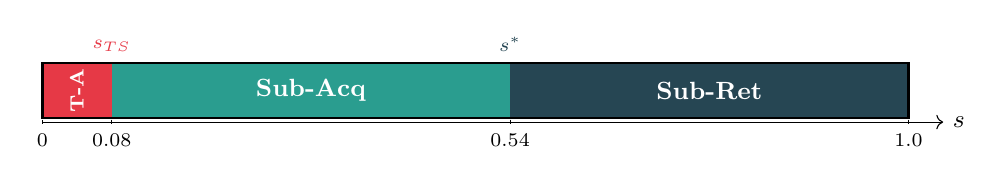
\begin{tikzpicture}[x=11cm,y=1cm]
    \fill[ottred]   (0,0)    rectangle (0.08,0.7);
    \fill[ottteal]  (0.08,0) rectangle (0.54,0.7);
    \fill[ottdark]  (0.54,0) rectangle (1.0,0.7);
    \draw[thick] (0,0) rectangle (1.0,0.7);
    \node[white,font=\scriptsize\bfseries,rotate=90] at (0.04,0.35) {T-A};
    \node[white,font=\small\bfseries]  at (0.31,0.35) {Sub-Acq};
    \node[white,font=\small\bfseries]  at (0.77,0.35) {Sub-Ret};
    \draw[->] (0,-0.05) -- (1.04,-0.05) node[right]{\small $s$};
    \foreach \x in {0,0.08,0.54,1.0} \draw (\x,-0.02)--(\x,-0.08);
    \node[below,font=\scriptsize] at (0,-0.08) {0};
    \node[below,font=\scriptsize] at (0.08,-0.08) {0.08};
    \node[below,font=\scriptsize] at (0.54,-0.08) {0.54};
    \node[below,font=\scriptsize] at (1.0,-0.08) {1.0};
    \node[ottred,font=\scriptsize,above] at (0.08,0.72) {$s_{TS}$};
    \node[ottdark,font=\scriptsize,above] at (0.54,0.72) {$s^{*}$};
  \end{tikzpicture}
  \end{center}
  \vskip0.2em
  \centering\footnotesize
  \begin{tabular}{l|l|l}
    市佔率區間 & 最適策略 & 經濟意義\\\hline
    $s\in[0,0.08]$    & \TA & 極早期試水;SVOD stage profit 為負,TVOD 低門檻拉新\\
    $s\in[0.08,0.54]$ & \SA & 主要成長階段;滲透定價,acquisition 動態邊際強\\
    $s\in[0.54,1.0]$  & \SR & 成熟期;retention 動態邊際支配,flat-rate bias 完全發揮\\
  \end{tabular}
  \vskip0.3em
  {\footnotesize $(T,R)$ 從未被選 —— TVOD 較低的人均收入使 retention 投資在任何 $s$ 皆不划算。}
\end{frame}

\begin{frame}{穩態與廠商不對稱:Incumbent Advantage}
  \begin{columns}[T]
    \column{0.54\textwidth}
      \centering\small
      \begin{tabular}{l|c|c|c}
        廠商類型 & $s_0$ & $s_{25}$ & 折現利潤\\\hline
        Newcomer\,(Apple TV+) & 0.05 & 0.505 & 79.56\\
        Mid-share\,(Disney+)  & 0.30 & 0.505 & 86.23\\
        Incumbent\,(Netflix)  & 0.65 & 0.505 & \textbf{97.41}\\
      \end{tabular}
      \vskip0.8em
      \begin{tikzpicture}[x=3.4cm,y=1.3cm]
        \draw[->] (0,0)--(1.05,0) node[right,font=\scriptsize]{$s$};
        \draw[->] (0,0)--(0,1.15) node[above,font=\scriptsize]{$V(s)$};
        \draw[rblue,very thick] plot[smooth,domain=0:1,samples=40,variable=\x]
              (\x,{0.15+0.95*\x*\x});
        \node[rblue,font=\scriptsize] at (0.6,0.95) {凸 $V(s)$};
      \end{tikzpicture}
    \column{0.46\textwidth}
      \begin{alertblock}{核心發現}
        三類廠商最終都收斂到同一穩態 $s_\infty\approx 0.505$,
        但 25 年累積折現利潤\textbf{相差約 22\%}。
      \end{alertblock}
      \footnotesize
      來源:價值函數 $V(s)$ 的\textbf{凸性} —— 早期高 $s$ 的累積利益因折現
      ($\beta^t$)而\textbf{不可挽回}。\\[0.4em]
      先進者享有追不回的折現利潤優勢 $\Rightarrow$ 解釋為何 Disney+、Apple TV+
      願意年虧十億美元也要\textbf{早期進場}。
  \end{columns}
\end{frame}

\begin{frame}{策略地圖 vs.\ 動態可達性的張力}
  修正雙重飽和 bug 後浮現的洞察:策略地圖預測 $s\ge0.54$ 應採 Sub-Ret,
  但\textbf{動態演化顯示新進廠商永遠到不了該區段}。
  \vskip0.3em
  \centering\small
  \begin{tabular}{l|c|c}
    策略(若永遠採用) & 假想穩態 $s^{*}$ & 是否 self-consistent?\\\hline
    Trans-Acq & $0.30/0.65=0.462$ & \rd{\ding{55}} 在 0.462 應切到 Sub-Acq\\
    Trans-Ret & $0.15/0.40=0.375$ & \rd{\ding{55}} 在 0.375 應切到 Sub-Acq\\
    \textbf{Sub-Acq} & $0.25/0.495=0.505$ & \textcolor{ottteal}{\textbf{\ding{51}} 在 0.505 仍在 Sub-Acq}\\
    Sub-Ret & $0.10/0.245=0.408$ & \rd{\ding{55}} 在 0.408 應切到 Sub-Acq\\
  \end{tabular}
  \vskip0.5em
  \begin{exampleblock}{洞察:Sub-Ret 是 Incumbent 專屬策略}
    \footnotesize
    只有 Sub-Acq 的假想穩態(0.505)與最適政策自洽 $\Rightarrow$ 唯一全域吸引子。
    Sub-Ret 只有 incumbent 在「市佔率下滑階段」會用;新進廠商從低 $s_0$ 自然演化\textbf{到不了}。
    對應現實:Netflix 2022 password-sharing crackdown 正是高 $s_0$ 下滑時點;
    Disney+/Apple TV+ 的 endgame 是 Sub-Acq 穩態。
  \end{exampleblock}
\end{frame}

\begin{frame}{結論的等級評估}
  \centering
  \begin{tabular}{c|l|l}
    等級 & 結論 & 穩健性來源\\\hline
    \textcolor{rblue}{\textbf{強}} & 存在策略轉換門檻 & 結構性($\beta>0$ 即成立)\\
    \textcolor{rblue}{\textbf{強}} & Incumbent advantage 的折現累積 & $V$ 的凸性\\
    \textcolor{rblue}{\textbf{強}} & 3-regime 結構 & 動態整合的湧現性質\\
    \textcolor{ottsand}{\textbf{中}} & Trans-Ret cell 從未被選 & 合理校準範圍內穩健\\
    \textcolor{ottsand}{\textbf{中}} & 內生穩態 $s_\infty$ & 飽和效應\\
    \rd{弱} & 具體門檻數值 & 依賴特定校準,勿過度宣稱\\
  \end{tabular}
  \vskip1em
  \begin{block}{解讀}
    結構性結論(門檻存在、incumbent advantage、三段結構)穩健;
    \textbf{具體數值}(0.08、0.54、0.505)依賴校準,僅作量級參考。
  \end{block}
\end{frame}

% =====================================================================
\section{延伸模型與結果}
% =====================================================================

\begin{frame}{延伸一:多重穩態與路徑依賴}
  \begin{columns}[T]
    \column{0.42\textwidth}
      \footnotesize
      \textbf{Baseline:單一穩態。}從 51 個起點全收斂到唯一 $s_\infty\approx0.505$
      ($f(s)$ 單調、斜率 $<1$,與對角線僅交叉一次)。\\[0.5em]
      \textbf{引入留存網路外部性:}
      \[ \rho(P,C,s)=\rho_0+\delta_P+\delta_C+\kappa\, s \]
      平台越大、留客率越高 $\Rightarrow$ $\kappa$ 上升時出現多重穩態。
      \vskip0.3em
      \centering\scriptsize
      \begin{tabular}{c|c|l}
        $\kappa$ & \#fp & 不動點\\\hline
        0.0 & 1 & 0.388\\
        0.2 & 1 & 0.450\\
        \textbf{0.3} & \textbf{3} & 0.507,\,0.909,\,0.976\\
        0.4 & 2 & 0.909,\,0.960\\
      \end{tabular}
    \column{0.58\textwidth}
      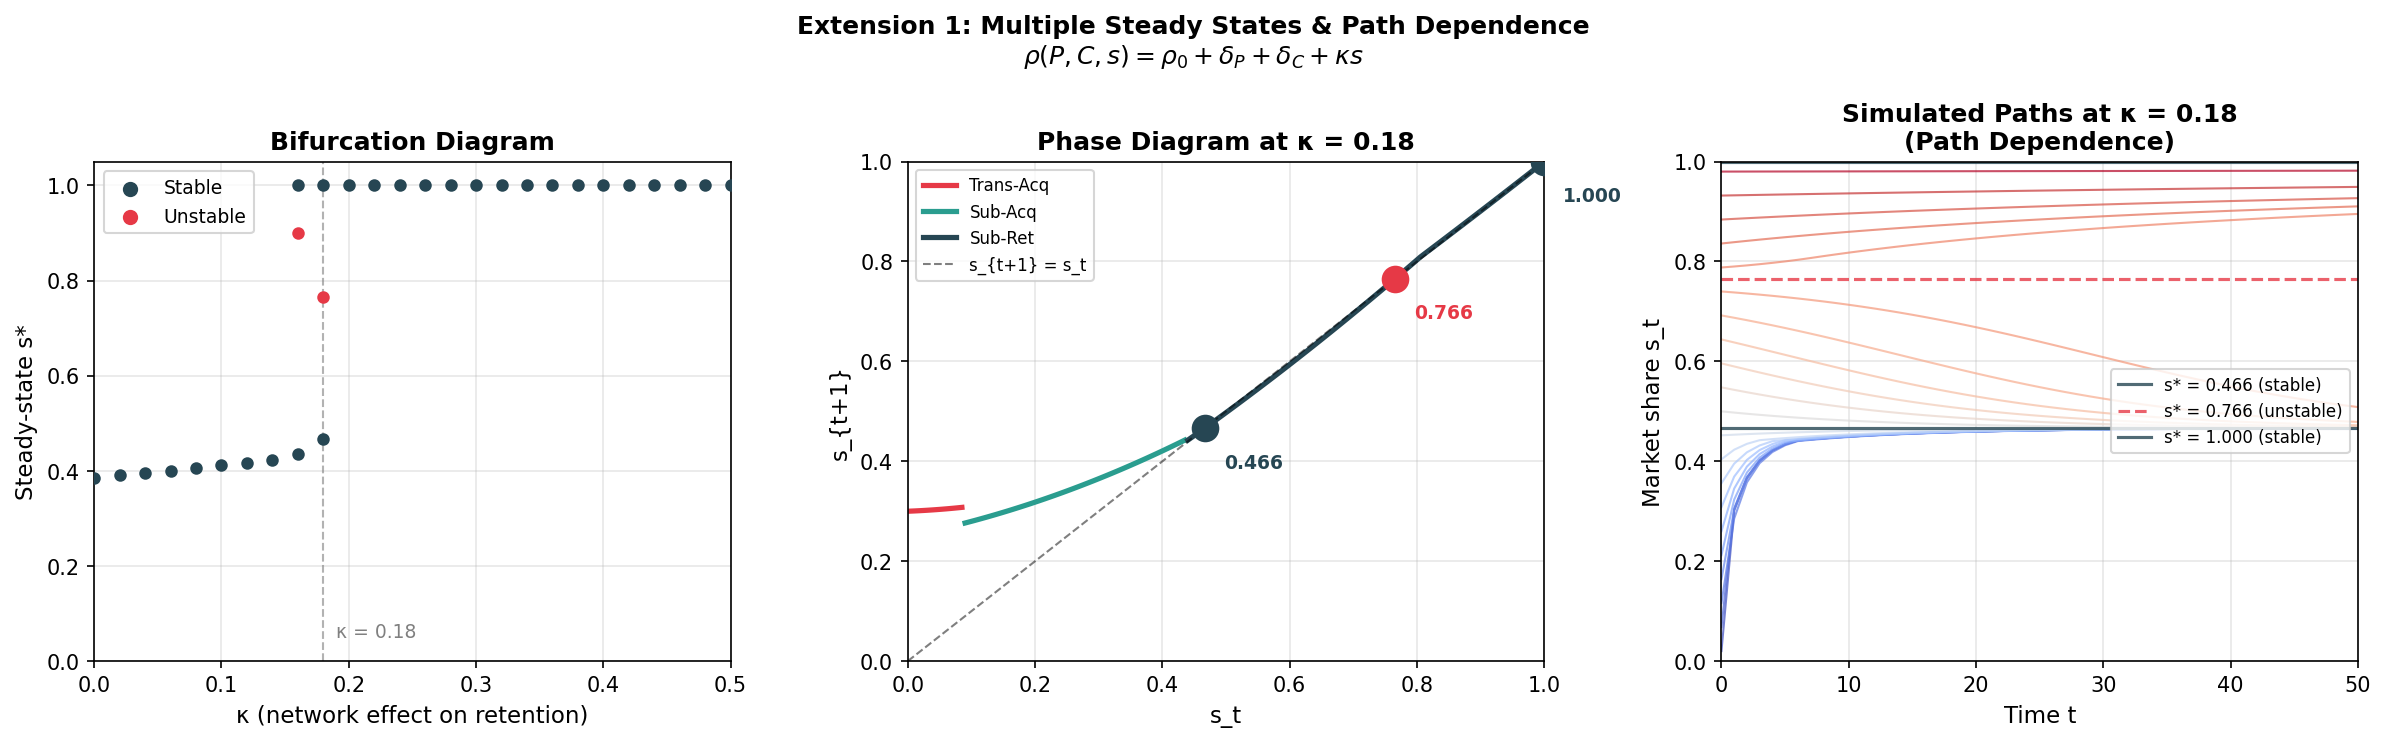
\includegraphics[width=\linewidth]{extension1_multi_steady.png}\\
      {\scriptsize 分歧圖(左)、相圖(中)與多起點模擬(右):
       saddle-node bifurcation 後出現低/高雙穩態與不穩定臨界點。}
  \end{columns}
  \vskip0.2em
  \begin{alertblock}{洞察:Critical Mass 與 Path Dependence}
    \footnotesize 當留存網路外部性夠強,\textbf{初始市場地位決定長期結果}:小平台可能被困在低均衡,
    即使高均衡存在。呼應 Rohlfs (1974) 臨界質量、Arthur (1989) lock-in、David (1985) QWERTY。
  \end{alertblock}
\end{frame}

\begin{frame}{延伸二:連續 effort 配置}
  把客群維度從 binary 改為\textbf{連續比例}:retention effort $e\in[0,1]$,acquisition $1-e$。
  \begin{block}{關鍵數學事實:凹性決定結果性質}
    \footnotesize
    effort $\to$ rate 的\textbf{凹性}決定一切。線性對應 $\Rightarrow$ 目標對 $e$ 線性 $\Rightarrow$
    最適必為 corner($e\in\{0,1\}$)$\Rightarrow$ 退化回 binary。唯有\textbf{凹對應}(邊際遞減)
    才有 interior solution $\Rightarrow$ 廠商最適地「同時做兩者」。曲率參數 $\gamma$:$\gamma{=}1$ 線性、$\gamma{<}1$ 凹。
  \end{block}
  \begin{columns}[T]
    \column{0.46\textwidth}
      \centering\scriptsize
      \begin{tabular}{c|ccccc}
        $s$ & 0.3 & 0.4 & 0.5 & 0.6 & 0.7\\\hline
        $e^{*}$ & 0.12 & 0.25 & 0.43 & 0.63 & 0.80\\
        配置 & 88\%A & 75\%A & 57\%A & 62\%R & 80\%R\\
      \end{tabular}
      \vskip0.3em {\scriptsize 收斂 399 次迭代;$e^{*}(s)$ 平滑遞增,$s\approx0.52$ 處 50/50。}
    \column{0.54\textwidth}
      \begin{exampleblock}{三個核心發現}
        \footnotesize
        \textbf{(1) 開關變曲線}:baseline 的瞬跳 $\to$ 平滑滑動,更貼近現實。\\
        \textbf{(2) 連續控制價值更高}:逐點 $V_{\text{cont}}\ge V_{\text{disc}}$,平均 $+12.87$,中段增益最大($+14$)。\\
        \textbf{(3) 曲率決定 corner vs.\ interior}:邊際遞減越強,內部解(同時做兩者)越多。
      \end{exampleblock}
  \end{columns}
\end{frame}

\begin{frame}{延伸三:成本設計的深化}
  baseline 把成本設為定值是較弱的一環。採 Min et al.\ (2016) 的
  \hl{飽和/規模依賴}成本(41 國電信實證):acquisition 隨市場飽和變貴、retention 隨客群規模上升。
  \begin{columns}[T]
    \column{0.5\textwidth}
      \centering\footnotesize
      \textbf{Discrete:門檻前移}\\[0.2em]
      \begin{tabular}{l|c|c}
        區間/指標 & OLD(定值) & NEW($s$-依賴)\\\hline
        Sub-Acq & [0.085,0.540] & [0.080,0.487]\\
        Sub-Ret & [0.542,1.0] & [0.490,1.0]\\
        主門檻 & 0.541 & \textbf{0.489} ($\downarrow$0.052)\\
        穩態 & 0.505 & 0.490\\
      \end{tabular}
    \column{0.5\textwidth}
      \begin{block}{四個 takeaway}
        \scriptsize
        \textbf{(1)} 定值成本系統性\textbf{低估}成熟廠商守成傾向(門檻前移 0.05)。\\
        \textbf{(2)} 連續控制對成本衝擊更穩健(穩態僅 $\downarrow$0.006 vs.\ discrete $\downarrow$0.015)。\\
        \textbf{(3)} convex cost 懲罰極端集中 $\Rightarrow$ 促進 diversification。\\
        \textbf{(4)} \hl{Dimension separation}:成本只動客群維度(A/R),收費維度(T/S)由收入結構主導、幾乎不變。
      \end{block}
  \end{columns}
  \vskip0.2em
  {\footnotesize 對偶性:response 凹 $\Leftrightarrow$ cost 凸。acquisition cost 由 1.20 翻倍至 2.40,
   retention 由 0.80 升到 1.04,不對稱性直接來自 Min et al.}
\end{frame}

\begin{frame}{延伸四:競爭擴展(Stackelberg 賽局)}
  自然延伸:大小公司賽局 —— Leader(Netflix)先動,Follower(Apple TV+)觀察後反應。
  \begin{columns}[T]
    \column{0.5\textwidth}
      \begin{block}{模型結構}
        \footnotesize
        狀態 $(s_L,s_C)$,$s_L+s_C\le1$。轉移加入對手搶客項:
        \[ s_{C,t+1}=\rho s_C+\alpha(1-s_L-s_C)+\underbrace{\gamma s_L}_{\text{挖角}} \]
        兩個\textbf{耦合 Bellman},需交替更新(backward induction / MPE)。
      \end{block}
      \begin{alertblock}{與 minimax 的區別}
        \footnotesize OTT 為\textbf{非零和}:大公司流失的客戶不必然被小公司搶到(可流向「不看 OTT」),
        市場可同時擴大。故非 minimax,而是 Stackelberg / Markov Perfect Equilibrium。
      \end{alertblock}
    \column{0.5\textwidth}
      \begin{exampleblock}{預期洞察}
        \footnotesize
        \textbf{(1) 小公司 differentiation}:可能主打 TVOD 避開 SVOD 主戰場(Mubi、Criterion 等利基)。\\
        \textbf{(2) 大公司 deter vs.\ accommodate}:何時壓制對手成長 vs.\ 讓出市場、專注高 $s$ 利潤。\\
        \textbf{(3) 內生市場結構}:雙寡占/一家獨大/利基共生等均衡的內生產生。
      \end{exampleblock}
      \footnotesize 狀態 1D$\to$2D 約 $\times100$;operator 非 contraction(不保證收斂);
      務實簡化:採「myopic Follower」可回到 1D。
  \end{columns}
\end{frame}

% =====================================================================
\section{結論}
% =====================================================================

\begin{frame}{研究限制}
  \footnotesize
  \begin{enumerate}\itemsep3pt
    \item \textbf{樣本非純 OTT}:Iyengar (2011) 為行動電話、Datta (2015) 為 digital TV、Rao (2015) 為 iTunes 型;
          直接以 Netflix/Disney+ 校準的學術論文極少。
    \item \textbf{單一廠商假設}:可能\textbf{高估} retention 最適投入;建議以 reduced-form competitive intensity 參數模擬。
    \item \textbf{內容投資未明確進入模型}:Bernstein et al.\ (2022) 提醒內容是 retention 槓桿;建議將 content stock 作為次要狀態變數。
    \item \textbf{行為偏誤方向可能反轉}:flat-rate bias 在 2006 顯著,但 2023--2025 訂閱疲勞(Deloitte 2025:47\% 認為過貴)顯示可能反轉。
    \item \textbf{reduced-form 而非 structural}:$\rho,\alpha$ 為查表定值;以完整 sensitivity 與「3-regime 湧現性質」凸顯貢獻。
  \end{enumerate}
  \vskip0.2em
  {\footnotesize 校準誠實性:真正來自文獻的只有 $\delta_S{=}{+}0.105$(Iyengar 2011)與 $\beta{=}0.95$,其餘為設計性 baseline,需敏感度分析。}
\end{frame}

\begin{frame}{結論}
  \footnotesize
  \begin{enumerate}\itemsep2pt
    \item \textbf{三段策略地圖}:Trans-Acq($s{<}0.08$)$\to$ Sub-Acq($0.08{\le}s{<}0.54$)$\to$ Sub-Ret($s{\ge}0.54$),
          對應 OTT「試水 $\to$ 規模化拉新 $\to$ 成熟期留客」生命週期。
    \item \textbf{Incumbent advantage}:同穩態 $s_\infty\approx0.505$,但累積折現利潤相差約 22\%(源於 $V$ 凸性)。
    \item \textbf{Sub-Ret 為 incumbent 專屬}:只有 Sub-Acq 穩態自洽;新進廠商永遠停在 Sub-Acq。
    \item \textbf{多重穩態的可能}:引入留存網路外部性 $\kappa s$ 即出現 saddle-node bifurcation 與路徑依賴(臨界質量)。
    \item \textbf{連續 effort 配置}:sharp threshold $\to$ 平滑曲線;連續控制價值更高;「同時做兩者」的充要條件是邊際遞減。
    \item \textbf{成本設計深化}:飽和/規模依賴成本使廠商\textbf{更早}轉向 retention;成本只動客群維度(dimension separation)。
  \end{enumerate}
  \vskip0.4em
  \begin{exampleblock}{方法論貢獻}
    不在任何單一 stream,而在\hl{兩條 stream 的動態整合},以及整合後浮現的非平凡性質
    (3-regime 結構、策略地圖與動態可達性的張力、連續配置的平滑梯度、成本不對稱對守成傾向的放大)。
  \end{exampleblock}
\end{frame}

% ----------------------------- Appendix / Thanks -----------------------------
\appendix
\begin{frame}{附錄:核心模型速查}
  \small
  \begin{align*}
    \text{Bellman:}\quad & V(s)=\max_{a}\{\pi(s,a)+\beta V(s')\}\\
    \text{利潤:}\quad & \pi(s,a)=R(s,P)\,s-C(C)\\
    \text{收入:}\quad & R(s,S)=p_S=15,\quad R(s,T)=p_T(\varphi_0+\varphi_1 s)=2.5+2.5s\\
    \text{轉移:}\quad & s'=\rho(P,C)\,s+\alpha(P,C)\,(1-s)\\
    \text{留存:}\quad & \rho(P,C)=\rho_0+\delta_P+\delta_C\\
    \text{獲取:}\quad & \alpha(P,C)=\alpha_0+\tilde\delta_P+\tilde\delta_C\quad(\text{不依 } s)
  \end{align*}
  \centering $\beta=0.95$,\ 4 個離散 cell $(P,C)\in\{T,S\}\times\{A,R\}$,\ 201 格點 value iteration。
\end{frame}

\begin{frame}[plain]
  \vfill\centering
  {\color{rblue}\rule{0.5\textwidth}{1.4pt}}\\[0.8em]
  {\Large\bfseries\color{rblue} 謝謝聆聽 \quad Q\,\&\,A}\\[0.6em]
  {\footnotesize 線上影音串流平台之二維動態策略模型 $\cdot$ IEGT 2026}\\[0.6em]
  {\color{rblue}\rule{0.5\textwidth}{1.4pt}}
  \vfill
\end{frame}

\end{document}
